\documentclass[]{article}

\usepackage{amsmath}
\usepackage{graphicx}
\usepackage{url}

%opening
\title{AERO 626 Challenge Problem}
\author{Tim Woodbury}

\begin{document}

%\pagenumbering{gobble} % remove page numbers?

% Objectives
%	Present algorithms for 5 filters
%	Establish baseline sequential estimation performance, with measures of accuracy and consistency
%	Consider an advanced estimation case with ambiguous measurements and infrequent measurements
% Dynamic system
%	Governing equations
%	Bifurcation behavior
% Algorithms
%	EKF
%	UKF
%	etc
% Simulation overview
%	Performance and error metrics
%		MSE
%		NEES metric
%	Modification for bifurcated system
%		ENKF modifications
%		Error computation in the bifurcation case
% Results
%	Sequential case
%	Bifurcation case
% Conclusions

\maketitle

\section{Overview}

\section{Filter algorithms}

Five estimation algorithms are considered for the nonlinear sequential estimation problem: the Extended Kalman Filter (EKF), the Unscented Kalman Filter (UKF), the Sequential Importance Resampling (SIR) particle filter (PF), the Ensemble Kalman Filter (ENKF), and the Gaussian Mixture Model (GMM). For completeness, the algorithm governing each filter is described in the following sections.

\subsection{Extended Kalman filter}

The Extended Kalman filter is the most popular sequential estimation algorithm in the field of guidance, navigation, and control. Simply put, the EKF replaces the linear process and measurement influence matrices in the linear Kalman filter algorithm with the Jacobian of nonlinear governing functions evaluated at an aposteriori state estimate. The algorithm description is taken from Ref. \cite{crassidis}. The assumed prior estimate $\hat{x}(0)$, covariance $P(0)$, and dynamic system are of the following form:

\begin{align}
\hat{x}(0) = E[x_0] \\
P(0) = E[(\hat{x}(0)-x_0)(\hat{x}(0)-x_0)^T] \\
x_k = f(x_{k-1},t_{k-1}) + G_k w_k, w_k \sim N(0,Q_k) \\
y_k = h(x_k,t_k) + v_k, v_k \sim N(0,R_k)
\end{align}

The discrete propagation equations for the state and covariance follow:

\begin{align}
\hat{x}_{k}^- = f(\hat{x}_{k-1},t_{k-1}) \\
P_{k}^- = F_{k-1}P_{k-1}F_{k-1}^T + G_{k-1}Q_{k-1}G_{k-1}^T \\
F_{k-1} \equiv \frac{\partial f}{\partial x} (\hat{x}_{k-1},t_{k-1})
\end{align}

The update equations for the state and covariance, given a measurement $\tilde{y}_k$, are:

\begin{align}
\hat{x}_k = \hat{x}_k^- + K_k(\tilde{y}_k-h(\hat{x}_k^-)) \\
P_k = (I-K_kH_k)P_k^- \\
K_k \equiv P_k^- H_k^T (H_k P_k^- H_k^T + R_k)^{-1} \\
H_k \equiv \frac{\partial h}{\partial x} (\hat{x}_k^-,t_k)
\end{align}

The EKF has been shown to work well for a variety of systems, given that the estimate PDF remains well approximated by a Gaussian. Many studies have also shown that the UKF generally performs better for nonlinear systems, at the cost of slightly greater computational complexity.

\subsection{Unscented Kalman filter}

The UKF is based on the same idea as the EKF; extend the linear Kalman update to nonlinear systems in an approximate fashion. In the UKF, however, function Jacobians are no longer used; instead, a discrete set of ``sigma points'' are defined and passed through the propagation and update equations. The output points are used to evaluate the system covariances from their definitions.

The algorithm here is repeated from Wan\cite{wan2000}; for a complete algorithmic description including the value of the weights and other algorithm parameters, the reader is encouraged to review this resource, or one of numerous others in the literature. Define the augmented state vector $x^a \ \in \ \mathcal{R}^L$ as follows:

\begin{equation}
x^a_k = \begin{bmatrix}
x_k \\w_k \\v_k
\end{bmatrix} \equiv \begin{bmatrix}
x^x_k \\x^w_k \\x^v_k
\end{bmatrix}
\label{eq:xaug_ukf}
\end{equation}

In Eq. \ref{eq:xaug_ukf}, $x^x_k$, $x^w_k$, and $x^v_k$ are used as shorthand for the augmented state members associated with the state, process noise, and measurement noise. The $L \times 2L+1$ array of sigma points is defined as follows. Note that $\lambda$ is an algorithm parameter.

\begin{equation}
\chi^a_{k-1} = [\hat{x}^a_{k-1} \ \hat{x}^a_{k-1}\pm \sqrt{(L+\lambda)P_{k-1}^a}]
\end{equation}

Each sigma point is then propagated through the governing nonlinear equation as follows:

\begin{equation}
\chi^-_{k}(:,j) = f(\chi^x_{k-1}(:,j),t_{k-1}) + G_k \chi^w_{k-1}(:,j), \ \forall \ j
\label{eq:ukf_prop}
\end{equation}

The state and covariance apriori estimates are given as weighted averages of the sigma points:

\begin{align}
\hat{x}_k^- = \sum_{i=1}^{2L+1} W_i^m \chi^{x-}_k(:,i) \\
P_k^- = \sum_{i=1}^{2L+1} W_i^c (\chi^{x-}_k(:,i)-\hat{x}_k^-)(\chi^{x-}_k(:,i)-\hat{x}_k^-)^T
\end{align}

In a similar fashion, the update is performed by first passing the propagated sigma points through the measurement equation:

\begin{equation}
Y_k(:,j) = h(\chi^{x-}_k(:,j),t_k) + \chi^v_{k-1}(:,j)
\label{eq:ukf_expectation}
\end{equation}

The measurement covariance and state-measurement cross-correlation are evaluated as follows:

\begin{align}
\hat{y}_k \equiv \sum_{i=1}^{2L+1} W_i^m Y_k(:,i) \\
P_{yy} \equiv \sum_{i=1}^{2L+1} W_i^c (Y_k(:,i)-\hat{y}_k)(Y_k(:,i)-\hat{y}_k)^T \\
P_{xy} \equiv \sum_{i=1}^{2L+1} W_i^c (\chi^{x-}_k(:,i)-\hat{x}_k^-)(Y_k(:,i)-\hat{y}_k)^T
\end{align}

The Kalman update is then performed as follows:

\begin{align}
K_k \equiv P_{xy} P_{yy}^{-1} \\
\hat{x}_k = \hat{x}_k^- + K_k(\tilde{y}_k - \hat{y}_k) \\
P_k = P_k^- - K_kP_{yy}K_k^T
\label{eq:ukf_end}
\end{align}

This completes the algorithm description.

\subsection{Sequential importance resampling particle filter}

The essential function of a particle filter is to propagate a set of candidate states forward in time, evaluate the likelihood of a given measurement for each point, and weight the points so that they form a discrete-valued approximation to the true system density function. Repeated applications of the likelihood function tend to reduce the weight associated with most particles to essentially zero, a phenomenon referred to as particle degeneracy. This phenomenon can be overcome in part by judicious application of resampling; sampling new particles from the aposteriori density function.

The SIR algorithm employed in this work is found in Ref. \cite{arulampalam}. The density function is approximated by a set of weights $\omega^{i}_k$ and points $x^{i}_k$ as follows:

\begin{equation}
p_k(x) \approx \sum_{i=1}^{N_s} \omega^{i}_k \delta(x-x^{i}_k)
\end{equation}

For the particular dynamic system under consideration, the SIR algorithm may be written as follows:

\begin{enumerate}
\item Draw process noise values as $w^i_{k-1} \sim N(0,Q_k)$, then propagate each particle according to:
\begin{equation}
x_k^{i} = f(x_{k-1}^{i+},t_{k-1}) + G_k w^i_{k-1}
\label{eq:pf_eqom}
\end{equation}
\item Update the weights according to:
\begin{align}
v_k^i \equiv \tilde{y}_k - h(x_k^i,t_k) \\
\omega_k^i = p(v_k^i)
\end{align}
\item Normalize the weights to sum to one
\item Resample all points
\end{enumerate}

The resampling algorithm is expanded below:

\begin{itemize}
\item Initialize the CDF as: $c_1 = 0$
\item For $i = 2:N_s$
	\begin{itemize}
	\item Construct the CDF according to: $c_i = c_{i-1} + \omega_k^i$
	\end{itemize}
\item $i = 1$
\item Draw a starting point: $u_1 \sim \mathcal{U}[0,N_s^{-1}]$
\item For $j = 1:N_s$
\begin{itemize}
	\item Move along the CDF: $u_j = u_1 + N_s^{-1}(j-1)$
	\item While $u_j > c_i$
		\begin{itemize}
		\item $i = i+1$
		\end{itemize}
	\item Assign sample: $x_k^{j+} = x_k^i$
	\item Assign weight: $\omega_k^{j+} = N_s^{-1}$
\end{itemize}
\end{itemize}

The new particles $x_k^{j+}$ are used in the propagation step of Eq. \ref{eq:pf_eqom}. The expectation and covariance at any time may be computed from the discrete PDF as follows:

\begin{align}
E[x_k] \equiv \mu_k \approx \sum_{i=1}^{N_s} \omega^{i}_k x^{i}_k \\
E[(x_k-\mu_k)(x_k-\mu_k)^T] \approx \sum_{i=1}^{N_s} \omega^{i}_k (x^i_k - \mu_k)(x^i_k - \mu_k)^T
\end{align}

\subsection{Ensemble Kalman Filter}

The Ensemble Kalman Filter attempts to address two limitations associated with the EKF: (1) the need to store and propagate a covariance matrix in time; (2) the approximation of the nonlinear system by the linearized system \cite{evensen}. The ENKF is a particle method; it relies on the propagation of a selection of points with random sampling to approximate the effects of process and measurement noise. Instead of using a weighted approximation to the PDF, the ENKF performs a Kalman update on each point in the ensemble, and the resulting set of points are treated in a Monte Carlo sense as approximating the true system PDF. The ENKF uses the same basic algorithm as the UKF, except the set of sigma points is replaced by an ensemble of points with associated random process and measurement noise.

Let the ensemble of points at time $t_k$ be in the array $\gamma_k \ \in \ \mathcal{R}^{n \times N_s}$, where $n$ is the dimension of the state and $N_s$ is the ensemble size. An augmented ensemble with the process and measurement noise may be assembled as follows:

\begin{equation}
\gamma^a_k = \begin{bmatrix}
\gamma_k \\
w^{(1)}_k & w^{(2)}_k & \dots & w^{(N_s)}_k \\
v^{(1)}_k & v^{(2)}_k & \dots & v^{(N_s)}_k
\end{bmatrix}
\label{eq:enkf_augmented}
\end{equation}

In Eq. \ref{eq:enkf_augmented}, the process and measurement noise members are drawn from the underlying distributions (which are assumed zero-mean Gaussian here, but need not be in general). The UKF propagation and update equations of Eq. \ref{eq:ukf_prop}, \ref{eq:ukf_expectation}-\ref{eq:ukf_end} may then be used with one additional change. The mean weights $W^m_i$ and covariance weights $W^c_i$ are replaced by the constants used in the definitions of sample mean and covariance; $W^m_i \leftarrow \frac{1}{N_s}$, $W^c_i \leftarrow \frac{1}{N_s-1}$. The ENKF propagation consists only of propagating each point in the ensemble, using randomly drawn process noise:

\begin{equation}
x_{k+1}^{(i)-} = f(x_{k}^{(i)},t_k) + G_k w_{k}^{(i)} \ w_k^{(i)}, \sim N(0,Q_k)
\end{equation}

The ENKF update step is readily accomplished using the particle approximation of the measurement covariance $P_{yy}$, the cross-covariance $P_{xy}$, and the usual Kalman update:

\begin{align}
\hat{x}_k^{-} = \frac{1}{N_s} \sum_{i=1}^{N_s} x_{k}^{(i)-} \\
\hat{y}_k^{(i)-} = h(x_{k}^{(i)-},t_k) + v_k^{(i)}, \ v_k^{(i)} \ \sim \ N(0,R_k) \\
\hat{y}_k^{-} = \frac{1}{N_s} \sum_{i=1}^{N_s} y_k^{(i)-} \\
P_{yy} \equiv \frac{1}{N_s-1} \sum_{i=1}^{N_s} ({y}_k^{(i)-} - \hat{y}_k^{-})({y}_k^{(i)-} - \hat{y}_k^{-})^T \\
P_{xy} \equiv \frac{1}{N_s-1} \sum_{i=1}^{N_s} ({x}_k^{(i)-} - \hat{x}_k^{-})({y}_k^{(i)-} - \hat{y}_k^{-})^T \\
K_k \equiv P_{xy} P_{yy}^{-1} \\
\hat{x}_k^{(i)} = \hat{x}_k^{(i)-} + K_k(\tilde{y}_k - \hat{y}_k^{(i)-}) \\
\hat{x}_k = \frac{1}{N_s} \sum_{i=1}^{N_s} x_{k}^{(i)} 
\label{eq:xest_enkf}  \\
\end{align}

\subsection{Adaptation in the Ensemble Kalman filter}

Because the ENKF estimates are finite sums, it is possible to adjust the size of the ensemble based on the convergence behavior of the sum. This has the potential to number of wasted computations by reducing the ensemble size when extra points are not producing better estimates. A simple, ad hoc adaptation scheme is employed for limited comparison against the fixed-sized ENKF.

The adaptation scheme used is based upon the Frobenius norm of the covariance estimate. Let $|| X ||$ denote the Frobenius norm of matrix $X$. Let $P(N_s)$ denote the covariance approximation for $N_s$ ensemble points, where the covariance is determined as follows:

\begin{equation}
P(N_s) = \frac{1}{N_s-1} \sum_{i=1}^{N_s} ({x}_k^{(i)-} - \hat{x}_k^{-})({x}_k^{(i)-} - \hat{x}_k^{-})^T
\end{equation}

For a given ensemble size, the performance with one fewer ensemble member is evaluated. The performance metric $J = || P(N_s) - P(N_s-1)||/||P(N_s)||$ is considered. If $J$ is greater than a pre-defined tolerance, the ensemble size is reduced by eliminating one point, and the process repeats until convergence is achieved. If $J$ is greater than the tolerance, then a new point is sampled from the current best approximation to the mean and covariance. The new metric $J = || P(N_s+1) - P(N_s) ||/||P(N_s+1)||$ is considered. If $J$ is less than the tolerance, the new point is added, and the algorithm keeps adding points until tolerance is achieved; otherwise, the algorithm stops and the ensemble size is unchanged. 

This algorithm is not very efficient. It might be improved by not updating the ensemble size with every measurement, by integrating the ensemble adaptation with the finite covariance computation, or by attempting to extrapolate to the ``correct'' sample size, eliminating many repetitions of the algorithm. The algorithm is listed below for clarity:

\begin{itemize}
\item For a given initial ensemble size $N_s$:
	\begin{itemize}
	\item Evaluate the state covariance $P(N_s)$
	\item Remove one point in the ensemble arbitrarily and evaluate $P(N_s-1)$.
	\item Evaluate $J = \frac{|| P(N_s) - P(N_s-1)||}{||P(N_s)||}$
	\item If $J < \mathrm{tol}$
		\begin{itemize}
		\item While $J < \mathit{tol}$
			\begin{itemize}
			\item $N_s = N_s - 1$
			\item Remove one point in the ensemble arbitrarily and evaluate $P(N_s-1)$.
			\item Evaluate $J = \frac{|| P(N_s) - P(N_s-1)||}{||P(N_s)||}$
			\end{itemize}
		\end{itemize}
	\item Else:
		\begin{itemize}
		\item While $J > \mathit{tol}$
			\begin{itemize}
			\item Sample one point from current $\hat{x}$ and evaluate $P(N_s)$.
			\item $N_s = N_s + 1$
			\item Evaluate $J = \frac{|| P(N_s) - P(N_s+1)||}{||P(N_s+1)||}$
			\end{itemize}
		\end{itemize}
	\item Return
	\end{itemize}
\end{itemize}

The adaptive ENKF, or AENKF, is evaluated in a limited number of cases, mainly so its accuracy and the ensemble size can be compared against the standard ENKF.

\subsection{Gaussian mixture models}

The implementation of the Gaussian mixture model (GMM) is based on Ref. \cite{alspach}. The algorithm is repeated here for completeness. The prior density function is approximated as a sum of multivariate Gaussians with normalizing weights $\alpha_{ki}^{'}$ as follows:

\begin{align}
	p(x_k | y_k) = \sum_{i=1}^{\chi_k} \alpha_{ki} \eta(x_k-a_{ki},P_{ki}) \\
	\eta(a,P) \equiv \frac{1}{\sqrt{(2\pi)^n \mathrm{det}(P)}} e^{-\frac{1}{2} a^T P^{-1} a} \\
	\sum_{i=1}^{\chi_k} \alpha_{ki} = 1
\end{align}

For a discrete-time dynamic system with state influence function $x_{k+1} = f(x_k) + G_k w_k,w_k \sim N(0,Q_k)$, the individual Gaussian filters are propagated using the Extended Kalman Filter update for the means $a_{ki}$ and the covariances $P_{ki}^{'}$:

\begin{align}
	p(x_{k} | y_{k-1}) = \sum_{i=1}^{\chi_{k}^{'}} \alpha_{ki}^{'} \eta(x_{k}-a_{ki}^{'},P_{ki}^{'}) \\
	\chi_{k}^{'} = \chi_{k-1} \\
	\alpha_{ki}^{'} = \alpha_{(k-1)i} \\
	a_{ki}^{'} = f_k(a_{(k-1)i})\\
	P_{ki}^{'} = F_{ki}P_{(k-1)i}F_{ki}^T + G_{k} Q_k G_{k}^T \\
	F_{ki} \equiv \frac{\partial f_k}{\partial x} (a_{(k-1)i})
\end{align}

The update equations assume a nonlinear measurement of the form $y_k = h(x_k) + n_k, n_k \sim N(0,R_k)$. The aposteriori density function is approximated as follows:

\begin{align}
	p(x_{k} | y_{k}) = \sum_{i=1}^{\chi_{k}} \alpha_{ki} \eta(x_k-(a_{ki}^{'}+K_{ki}(y_k-h_k(a_{ki}^{'})),P_{ki}) \\
	\chi_k \equiv \chi_{k}^{'} \\
	P_{ki} \equiv P_{ki}^{'} - K_{ki} H_{ki} P_{ki}^{'} \\
	K_{ki} \equiv P_{ki}^{'} H_{ki}^T (H_{ki} P_{ki}^{'} H_{ki}^T + R_k)^{-1} \\
	\alpha_{ki} \equiv \frac{\alpha_{ki}^{'} \beta_{ki}}{\sum_{j=1}^{\chi_k} \alpha_{kj}^{'} \beta_{kj} } \\
	\beta_{kj} \equiv \eta(y_k - h_k(a_{kj}),H_{kj}P_{kj}^{'}H_{kj}^T + R_k)
\end{align}

This completes the description of the basic algorithm. Initialization of the prior is not addressed in Ref. \cite{alspach}. Two schemes are employed in the current work:

\begin{enumerate}
	\item Initialization of the means $a_{ki}$ to the sigma points used by the Unscented Kalman Filter
	\item Monte Carlo selection of the initial means
\end{enumerate}

In each case, the initial covariances $P_{0i}$ are selected to satisfy a prior Gaussian proposal with mean $\mu(0)$ and covariance $P(0)$. The mean and covariance of the initial distribution are computed as follows:

\begin{align}
	\mu \equiv E(x_k) = \sum_{i=1}^{\chi_k} \alpha_{ki} a_{ki} \\
	cov(x_k) = \sum_{i=1}^{\chi_k} \alpha_{ki} (P_{ki} + (a_{ki}-\mu)(a_{ki}-\mu)^T) \label{eq:cov_gmm}
\end{align}

Eq. \ref{eq:cov_gmm} represents an underconstrained system. By specifying that the initial distributions have equal covariance, the expression can be made tractable and solved for $P_{0}$:

\begin{equation}
	P_{0} = P(0) - \sum_{i=1}^{\chi_k} (\alpha_{ki}(a_{ki}-\mu)(a_{ki}-\mu)^T)
	\label{eq:P0_gmm}
\end{equation}

One practical note: astute readers will observe that the sum in Eq. \ref{eq:P0_gmm} with equal weights matches the statistical definition of the covariance (to within a small bias in the weights). Depending on the number of initial points and their distribution, the value of $P_{0}$ may not satisfy the requirement of positive definiteness for the covariance matrix. To ensure positive definiteness, $P_{0}$ is processed additionally by taking the absolute value of all members, and setting the diagonal elements to zero, to ensure the determinant remains positive.

The initial weights are initially set equal to one another, $\alpha_{ki} = \chi_k^{-1}$. It should be observed that for a unimodal near-Gaussian system, the algorithm will collapse to the Extended Kalman filter after a few iterations, with the means all concentrated near a single point. (This assumes that the initial means are all within the region of convergence for the EKF algorithm.) In the dynamics considered in the following section, the GMM is intended to address the case of bimodality in the propagated density function. The GMM is of most interest as an alternative to the PF and ENKF for handling multi-modality of the density.

\section{Governing equation and bifurcation time}

The system dynamics are governed by Eq. \ref{eq:eqom}, given below. The system consists of a cubic nonlinearity with white-noise and cosine forcing terms. For the purposes of estimation, the cosine forcing term is considered ``unknown''; that is, the magnitude may be known but the exact form cannot be used in the system propagation equation. Therefore, in practice both the white-noise term and the cosine forcing terms are lumped into a single process noise term that must encapsulate both sources.

\begin{align}
\ddot{x} = x - \epsilon x^3 + a_0 \cos{\omega_t t} + w(t) \label{eq:eqom} \\
w(t) \sim N(0,q)
\end{align}

\subsection{System parameters and measurement model}

The system measurement model is given as follows:

\begin{equation}
y_k = x_k + n_k, n_k \sim N(0,r)
\end{equation}

System measurements occur at discrete times $t_k = kT$. The total set of parameters that govern system behavior are defined below:

\begin{itemize}
\item $\epsilon = 0.01$
\item $a_0 = 0.5$
\item $\omega_t = 1.25$
\item $q = 1.0$
\item $r = 1.0$
\item $T \ \in \ [0.1,1.0]$
\end{itemize}

In addition, for numerical convenience in simulating the system dynamics, the process noise $w(t)$ is discretized at a fixed rate and held piecewise constant between samples. This effectively transforms as follows:

\begin{equation}
w(t) \rightarrow w_k \sim N(0,qT_s), t_k \leq t \leq t_{k+1}
\end{equation}

The dynamic uncertainty discretization time is taken as $T_s = 0.001$, which is an order of magnitude smaller than any of the measurement sample times used later.

\subsection{Bifurcation}

One feature of interest for the system is its equilibria: the unforced system has roots at $x = 0, \pm \sqrt{\frac{1}{\epsilon}}$. The roots at $\pm \sqrt{\frac{1}{\epsilon}}$ are attractive; the root at the origin is repulsive. The net effect is that, when propagated forward for a long enough time, a probability density initially centered at the origin will bifurcate into two distributions, roughly centered around the attractive equilibria. It is of interest to determine the bifurcation time, in examining the effectiveness of various filters.

Bifurcation time is analyzed with no forcing ($a_0 = 0$) by performing simulating a number of points from a normal distribution about the origin, then propagating forward in time. Results are plotted, and the bifurcation time estimated qualitatively. Fig. \ref{fig:bifurcation_animate_1} shows the development of the system bifurcation from its initial condition. The unforced motion is also shown by plotting the system after 9.5 seconds of development. From these plots, it is clear that bifurcation appears qualitatively on the order of a second or so. Therefore, the sample time of $10.0$ seconds is used to consider the bifurcated system in later study.

\begin{figure}[p!]
\centering
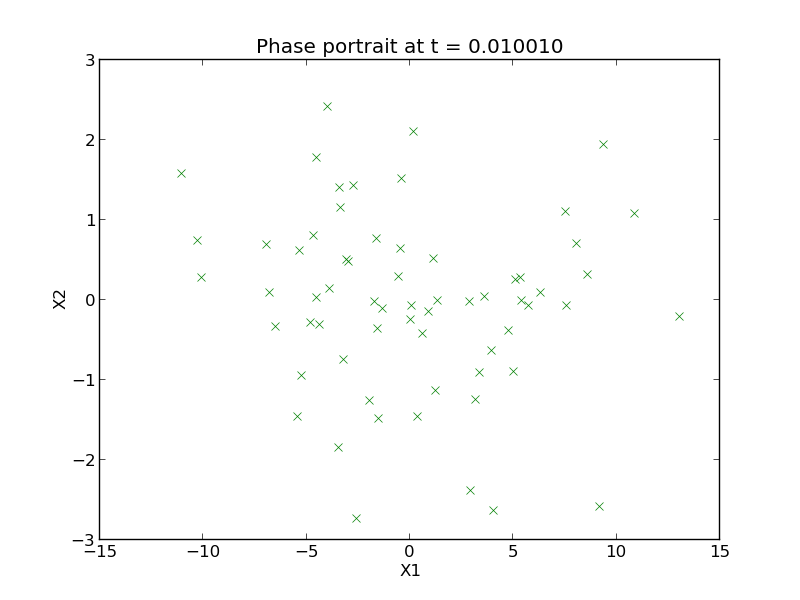
\includegraphics[height=0.275\textheight]{{../../challenge_problem/prelim_analysis/animate/anim_f1}.png}
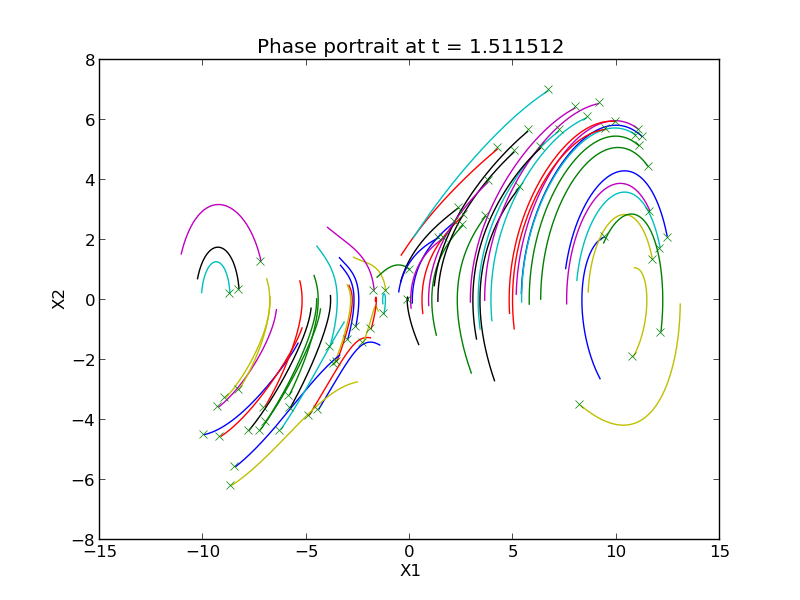
\includegraphics[height=0.275\textheight]{{../../challenge_problem/prelim_analysis/animate/anim_f151}.png}
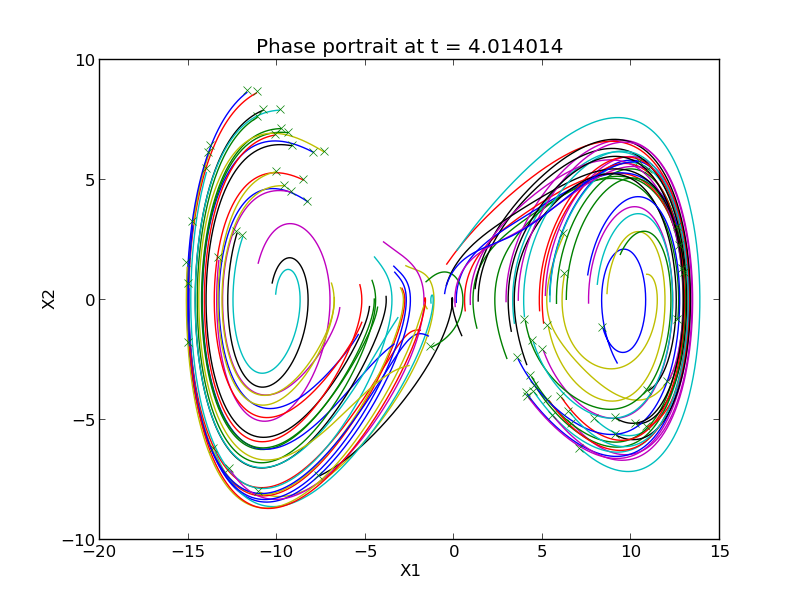
\includegraphics[height=0.275\textheight]{{../../challenge_problem/prelim_analysis/animate/anim_f401}.png}
\caption{Figures showing the development of the phase portrait of the distribution. 'x' is used to indicate the current condition of the state with the contours tracing the path history of the phase portrait. Axis labels: $X1$ indicates the position, $X2$ the speed. Top: Initially Gaussian points with position variance $2.0$ and speed variance $1.0$. Middle: Condition of the sustem after 1.5 seconds; clear separation between points in the phase portrait is visible. Bottom: Development of the system after several seconds, showing separation of points.}
\label{fig:bifurcation_animate_1}
\end{figure}

It is clear that so long as position is measured, at least one state of the bimodal system can be estimated in a stable fashion. It is of greater interest to consider the case where measurements provide limited or ambiguous information about the states under consideration. Therefore, in the bimodality study, measurements of the form $y = x_1^2$ are considered. To exaggerate the effect of the bimodality on the system, the process and measurement noise are each reduced by a factor of 100; this ensures that the system estimates tend to cluster about two candidate solution states, rather than spreading over a domain unimodally.

%A test for multimodality is performed using smoothed kernel density estimates (KDEs). The procedure is outlined briefly in the following subsection.

\subsection{Test for multimodality}

The test for multimodality is Silverman's\cite{silverman}; for implementation, reference is also made to \cite{adereth}. The KDE is a method of nonparametric estimation of a density function. The KDE for a particular kernel $K(.)$ is defined for samples $\chi = \{ X_1,X_2,...X_n \}$ as follows:

\begin{equation}
\hat{f}(x;h) = \frac{1}{nh} \sum_{i=1}^{n} K(\frac{x-X_i}{h})
\label{eq:kde_def}
\end{equation}

In Eq. \ref{eq:kde_def}, $h$ is a smoothing parameter. The kernel function in general may take different forms, but the Silverman test uses a univariate normal distribution. For a given data set $\chi$, the number of modes in the data (determined by the number of local extrema) is monotonically decreasing with the value of the smoothing parameter, according to Silverman\cite{silverman}. So, a simple binary search can be used to determine the critical smoothing parameter $h_{crit}$ at which the KDE has a particular number of modes. The objective of the test is to if the distribution of the position and velocity states at a fixed time is unimodal; therefore, the smoothing parameter for which the KDE has only one extrema is sought.

One additional procedure is used in the test; smoothed bootstrap sampling. The test works by evaluating the significance of the null hypothesis that the underlying distribution is unimodal. If the significance is too small, the null hypothesis is rejected, and the distribution is assumed to be multimodal. Smoothed bootstrap sampling is used to evaluate the significance level. Bootstrap samples $X_i^*$ are drawn from the original data set $\chi = \{ X_1,X_2,...X_n \}$ as follows:

\begin{equation}
X_i^* = \frac{X_{j(i)} + h\epsilon_i}{\sqrt{1+h^2/\sigma^2}}, i \in [1,\dots,n]
\label{eq:smoothedBootstrap}
\end{equation}

In Eq. \ref{eq:smoothedBootstrap}, the sample $X_{j(i)}$ is selected uniformly with replacement. $\sigma$ is the sample standard deviation of the data. $\epsilon_i$ is a normally distributed random variable with uniform variance. The smoothed bootstrap samples are used to evaluate the null hypothesis that the distribution is unimodal with a critical KDE parameter $h_{crit}$; $N_b$ sets are drawn using smoothed bootstrap sampling, and the number of maxima of the resulting KDE with $h_{crit}$ are tabulated. The fraction of sets with only one maximum is taken to be the significance level of the null hypothesis.

The test procedure is summarized as follows:

\begin{enumerate}
\item Simulate $N_p$ Monte Carlo simulations for a fixed time
\item For each time $t^*$ in the simulation outputs:
\begin{enumerate}
	\item Collect the $N_p$ state values at $t = t^*$
	\item Compute the critical smoothing parameter $h_{crit}$ for which the KDE is unimodal
	\item Evaluate the probability that the distribution has one mode
	\begin{enumerate}
		\item Perform smoothed bootstrap sampling from the critical KDE $N_b$ times
		\item For each of the $N_b$ samples:
		\begin{enumerate}
			\item Evaluate the KDE with the critical smoothing parameter for the current sample. Record the number of modes.
		\end{enumerate}
		\item The fraction of unimodal KDEs is taken as the P-value for the test.	
	\end{enumerate}
\end{enumerate}
\end{enumerate}

\section{Simulation description}

The estimation algorithms are evaluated in Monte Carlo simulation. Two categories of simulation are conducted: (1) a typical sequential filtering problem, referred to as the \textbf{standard case}, with relatively frequent measurements and approximately unimodal state distributions; (2) a case where significant bifurcation occurs due to the system dynamics, with infrequent, ambiguous measurements. The latter is referred to as the \textbf{bifurcation case}. All five algorithms are tested in the first scenario; in the second scenario, only the ENKF, SIR PF, and GMM are considered (that is, those models that have the ability to model non-unimodal distributions).

This section describes the settings used in both the standard and bifurcation cases; presents the performance metrics used; and describes how the ENKF is modified to work with ambiguous measurements in the bifurcation case.

\subsection{Overview of simulations}

In the standard case, forcing functions of white noise only, cosine forcing only, and cosine forcing with white noise are considered. In addition, sample rates varying from 100 Hz to 1 Hz are considered. This broad sweep of parameters helps highlight the performance differences between the various filters.

In the bifurcation case, the process and measurement noise levels are reduced, and only the case of Gaussian white noise is considered. The sample period is increased to five seconds, allowing the system pdf more than enough time to bifurcate. The modified system parameters are listed below for completeness:
\begin{itemize}
\item $a_0 = 0.0$
\item $q = 0.01$
\item $r = 0.01$
\item $T = 5.0$
\end{itemize}

\subsection{Performance metrics}

\subsection{Bifurcation and filter updates}

The ``Kalman'' estimators - that is, the EKF, UKF, ENKF, and GMM - all depend upon some version of the Kalman update to incorporate measurements into the sequential estimate. The Kalman gain, in turn, depends on the value of the system covariance. For a multimodal system, the covariance is a poor indicator of the actual system density, and leads to extremely conservative answers. When position is measured, the Kalman update should still remain reasonably bounded, although estimates should be expected to be conservative.

When the measurement is ambiguous, such as position squared, then any given measurement can correspond to two candidate position states; this prevents the estimator from resolving the propagated state cleaned to an aposteriori estimate. What happens typically is that the covariance grows to cover the entire cloud of possible points, and the estimated state converges towards the origin.

To resolve this ambiguity, the filters must be modified to account for multimodality. The SIR and GMM are the exceptions. The PF makes no explicit assumptions about the underlying state density, so provided enough particles are modelled, the SIR update and resampling is expected to naturally retain the points that match the measurement well. The GMM explicitly models the system as a sum of Gaussians, whose update equations are independent of one another. As long as the underlying Gaussians bifurcate when the underlying system density does, then the update equations should naturally reflect only the ``local'' covariance about each mode.

The EKF and UKF cannot handle a multimodal distribution without fundamental modification. The ENKF naturally models the system as a particle distribution, so there is some hope of modifying the Kalman update. Specifically, a simple approach is to autonomously cluster the data after propagation, and use the covariance of each cluster to update the particles in each cluster. This is, in generally, an extremely challenging problem; for the particular system under consideration, the problem is made tractable by the knowledge that the system distribution should have either one or two modes.

\subsubsection{ENKF clustering process}

The clustering process is summarized as follows:

\begin{itemize}
\item Propagate the system ensembles as usual.
\item Compute candidate system covariances for the case of both one and two modes, using K-means to classify ensemble particles in the bimodal case.
\item Use the measurement liklihood to select either the unimodal or bimodal distribution. Perform the system update on all modes (either one or two) as appropriate.
\end{itemize}

A na\"{i}ve K-means algorithm is relatively simple to implement, but does require apriori knowledge of the number of clusters. The K-means algorithm used in this work is found in Ref. \cite{mackay2003}. Essentially, K-means initializes by randomly assigning $k$ points in a sample set to be the ``means,'' then assigns membership to each point in the sample set based on the minimum Euclidean distance to each mean. Means are then updated by taking the mean of each cluster, then repeating until convergence is satisfied. Here, convergence is satisfied when the norm of the change in every mean during the update is less than $10^{-2}$. K-means in general converges only to a locally optimal value, but this is felt to be sufficient for the system under consideration.

Automatically selecting between candidate unimodal or bimodal distributions is a challenge. The K-means algorithm alone does not yield any goodness-of-fit metrics. Statistical tests for comparing multiple candidate models are frequently complicated, and replicating a robust statistical test is beyond the scope of this paper. The Akaike information criterion (AIC) was considered as a candidate for discriminating between fits. However, AIC in practice was found to penalize the additional complexity of the bimodal fit so greatly that a unimodal distribution was almost always chosen. In the end, a simple, na\"{i}ve maximum likelihood criterion was used. The likelihood function $p(\tilde{y} | \hat{x})p(\hat{x})$ is evaluated at each point in the ensemble for both one and two modes\footnote{In the bimodal case, it is assumed that each particle has discrete membership in each mode. That is, if particle $\hat{x}_{ki}$ is clustered into mean $j$, its likelihood function depends only on the mean and covariance associated with mean $j$.}. Whichever case produces the largest maximum value of the PDF is taken as the model for Kalman update purposes. This is a simplistic approach, likely unsuitable for many more sophisticated problems, but in this work, it produces a reasonable balance in terms of sometimes producing one mode and sometimes producing two.

\subsubsection{Error computation for bifurcated systems}

When the system has bifurcated, computation of the errors is no longer straightforward. The PF and GMM both approximate the system as a weighted sum of individual distributions, so it is reasonable to take the value derived from the largest weight at any given time as the model estimate. This may not correspond to a maximum likelihood solution exactly, particularly for the GMM, but is much simpler to evaluate.

For the clustering ENKF, a similar approach is taken. If a bimodal distribution is detected, then the mean is chosen to maximize $p(\tilde{y}_k | \hat{x}_k)$. For the scalar measurements used here, this is equivalent to choosing the aposteriori estimate whose expectation is closest to the measurement.

\section{Results}

\subsection{Standard case}

For the standard case, results are broken into three sections, each corresponding to a different sample rate. The sample rates used are $0.1$, $0.01$, and $1.0$ seconds, corresponding to medium, fast, and slow sample rates. For each sample rate, 100 Monte Carlo simulations of 30 seconds each are performed for three different cases of unmodelled forcing: (1) Gaussian white noise, (2) cosine forcing, (3) Gaussian white noise and cosine forcing.

For the SIR PF, 200 particles are used in each filter. For the ENKF, ensembles of size 100 are used in the non-adaptive case. Filter process noise terms were tuned for each filter and forcing case individually. It should be noted that the distinction is made between the \textbf{filter process noise} and the \textbf{simulation process noise}, the former being a tuning parameter for filter performance, and the latter being a global setting that changes the behavior of the underlying system.

Two performance metrics are used. The first is mean squared error (MSE), computed for the position states $x_1$ and speed states $x_2$ individually as follows:

\begin{equation}
\mathrm{MSE}_i = \frac{1}{N} \sum_{j=1}^N (\hat{x}_j(i) - x_j(i))^2
\end{equation}

MSE is computed across all times and all Monte Carlo simulations as an average metric of accuracy. To evaluate the consistency of each filter, the normalized expectation of the error squared (NEES) is employed. NEES is computed at a given simulation time as follows:

\begin{equation}
\mathrm{NEES}(t_k) = (\hat{x}_k-x_k)^T P_k^{-1} (\hat{x}_k-x_k)
\end{equation}

NEES is employed in two ways: first, the average NEES across the Monte Carlo runs at each simulation time is plotted as a function of time; second, 95\% confidence bounds for the NEES are computed as in Ref. \cite{neesPaper}. The 95\% confidence bounds are used to evaluate the fraction of times at which the mean NEES exceeded the 95\% bounds (indicating overconfidence of the estimate) and fell below the 95\% bounds (indicating conservatism of the estimate). This process yields two scalars that indicate the fraction of time steps at which a given filter was overconfident or overly conservative.

\subsubsection{Medium sample rate}

Performance for the $0.1$ second sample period case are collected in Tables \ref{table:compare_case_1_sample_0}-\ref{table:compare_case_3_sample_0} and Figs. \ref{fig:nees_01_medium}-\ref{fig:nees_11_medium}. It is noted first that the MSE accuracy of the ``Kalman'' filters, the EKF, UKF, and ENKF, is very similar in each case, typically differing only in the second decimal place. For the case of purely Gaussian forcing, the UKF performs best, followed by the ENKF and EKF; however, the actual difference in errors is probably too small to be significant in application. For the case of cosine forcing, the EKF has lowest errors, followed by the ENKF and UKF; again, the difference in the three is quite small. With combined forcing, the EKF performs best, followed by the UKF and ENKF.

In each case, it should be noted that the EKF estimates are extremely conservative compared to the UKF and ENKF. Extensive tuning of the filter process noise term allowed the EKF to achieve essentially identical performance at this $T_s$, but produces conservative error bounds that may or may not be acceptable in practice. The UKF is much less conservative in the white noise forcing case. For the cosine forcing and mixed forcing cases, the UKF is conservative at some times and optimistic at others. This is a product of using a white-noise forcing model to capture the effects of a cosine forcing term. To achieve good error performance, the filter's process noise term must be set so that it is conservative when the cosine term is small, and optimistic when the cosine term is near its maximum. The ENKF suffers from the same limitation in using a white-noise forcing model to capture a cosine forcing term; however, the extra flexibility of the ENKF in capturing nonlinear effects limits the extrema of conservatism and optimism.

Performance for the SIR PF in terms of MSE is typically worse than that of the other filters. However, it is noted that the fraction of conservative and optimistic points for the SIR is typically lower than for the other filters, especially in the cosine forcing cases. That indicates something about the PF produces less precise, yet more consistent estimates. Perhaps the process noise and number of particles has a ``shotgun'' effect on the propagation stage; that is, the filter propagation produces a broad set of candidate states, which are more likely to have some particles in the correct states to capture the effects of the nonlinear forcing. The filter covariance settings used are considered to be conservatively large. However, at smaller filter covariances, the particle degeneracy problem became much more significant and often led to zero weights after a single propagation step. Improved  accuracy might be achieved with the SIR with the conservative covariance settings and larger numbers of particles.

It is noted that the GMM tracks the EKF performance in each case, but with slightly larger errors. This is to be expected; since Monte Carlo initialization of the GMM is used with the standard EKF update for each Gaussian in the mixture, the GMM essentially converges to the EKF within a few updates. The GMM has extra covariance built into the initialization step, which causes the slightly larger overall MSEs.

Figs. \ref{fig:nees_01_medium}-\ref{fig:nees_11_medium} reflect the underlying differences between the different forcing environments. Performance for the tuned filters in any single forcing case is qualitatively similar; for instance, in Fig. \ref{fig:nees_01_medium}, each filter starts at a large initial mean NEES, due to the large initial covariance, and then decreases within about 10 seconds toward an apparent steady-state final value, with some oscillation. The UKF history is little ``tighter'' than the EKF, reflecting the improved consistency of the UKF. In Figs. \ref{fig:nees_10_medium} and \ref{fig:nees_11_medium}, on the other hand, the time histories are highly oscillatory, with a period reflecting that of the driving cosine forcing. These figures should make clear the limitation of using a white-noise forcing model to capture a nonlinear forcing term; the best-tuned filters have oscillate between conservative and optimistic.

%************************************************
% Performance table at Ts =  0.100000 with namebit 1
\begin{table}[h!]
\centering
\begin{tabular}{|c|c|c|c|c|}
\hline
Filter & $\mathrm{MSE}_1$ & $\mathrm{MSE}_2$ & Conservative fraction & Optimistic fraction \\
\hline
EKF &  0.09895 &   0.1252 &   0.7043 &        0 \\
\hline
ENKF &   0.0946 &   0.1206 &   0.5548 &        0 \\
\hline
AENKF &   0.1488 &   0.2547 &   0.2871 &        0 \\
\hline
GMM &   0.1305 &    0.172 &   0.7841 & 0.003322 \\
\hline
UKF &  0.09088 &   0.1169 &   0.4385 &  0.03655 \\
\hline
SIR &   0.1634 &   0.2738 &   0.1584 &   0.1188 \\
\hline
\end{tabular}
\caption{Performance metrics comparison of all filters with $T_s$ = 0.10 sec and Gaussian forcing term}
\label{table:compare_case_1_sample_0}
\end{table}


%************************************************
% Performance table at Ts =  0.100000 with namebit 2
\begin{table}[h!]
\centering
\begin{tabular}{|c|c|c|c|c|}
\hline
Filter & $\mathrm{MSE}_1$ & $\mathrm{MSE}_2$ & Conservative fraction & Optimistic fraction \\
\hline
EKF &   0.1444 &   0.2846 &   0.6977 &        0 \\
\hline
ENKF &   0.1455 &   0.2856 &   0.5249 &        0 \\
\hline
AENKF &   0.3373 &    1.936 &   0.0396 &   0.1188 \\
\hline
GMM &   0.1521 &   0.3213 &    0.206 &    0.113 \\
\hline
UKF &   0.1468 &   0.2898 &   0.1528 &    0.289 \\
\hline
SIR &   0.2694 &    1.171 &   0.0396 &        0 \\
\hline
\end{tabular}
\caption{Performance metrics comparison of all filters with $T_s$ = 0.10 sec and cosine forcing term}
\label{table:compare_case_2_sample_0}
\end{table}


%************************************************
% Performance table at Ts =  0.100000 with namebit 3
\begin{table}[h!]
\centering
\begin{tabular}{|c|c|c|c|c|}
\hline
Filter & $\mathrm{MSE}_1$ & $\mathrm{MSE}_2$ & Conservative fraction & Optimistic fraction \\
\hline
EKF &   0.1381 &    0.277 &   0.7475 &        0 \\
\hline
ENKF &    0.142 &   0.2871 &   0.2193 &   0.1063 \\
\hline
AENKF &    4.459 &    13.75 &  0.01329 &   0.6545 \\
\hline
GMM &   0.1467 &   0.3121 &   0.2193 &  0.08638 \\
\hline
UKF &   0.1402 &   0.2813 &   0.1694 &   0.2691 \\
\hline
SIR &   0.1599 &   0.3126 &  0.04651 &   0.1196 \\
\hline
\end{tabular}
\caption{Performance metrics comparison of all filters with $T_s$ = 0.10 sec and Gaussian and cosine forcing terms}
\label{table:compare_case_3_sample_0}
\end{table}

\begin{figure}[p!]
\centering
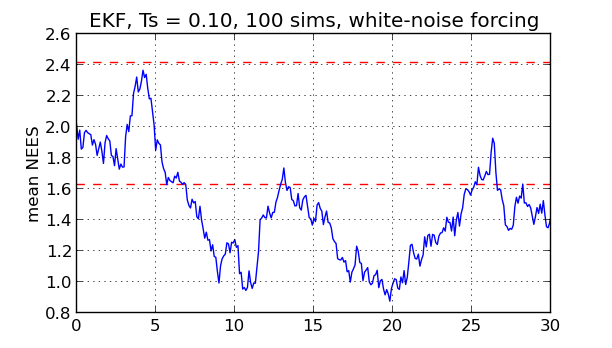
\includegraphics[width=0.49\textwidth]{../../challenge_problem/trials/nees_ekf_sims_01_medium}
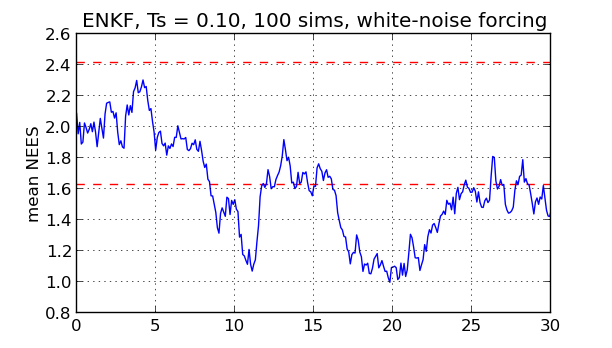
\includegraphics[width=0.49\textwidth]{../../challenge_problem/trials/nees_enkf_sims_01_medium}
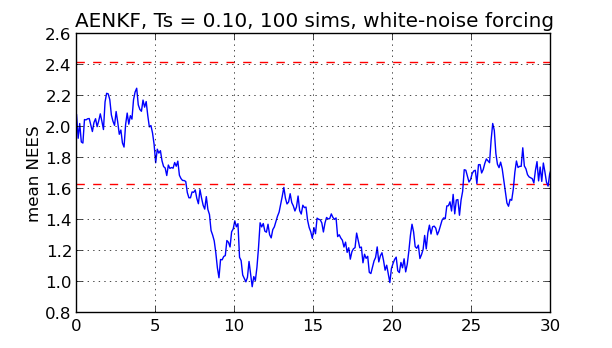
\includegraphics[width=0.49\textwidth]{../../challenge_problem/trials/nees_aenkf_sims_01_medium}
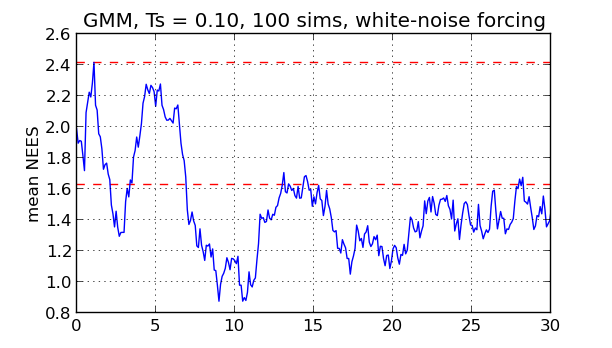
\includegraphics[width=0.49\textwidth]{../../challenge_problem/trials/nees_gmm_sims_01_medium}
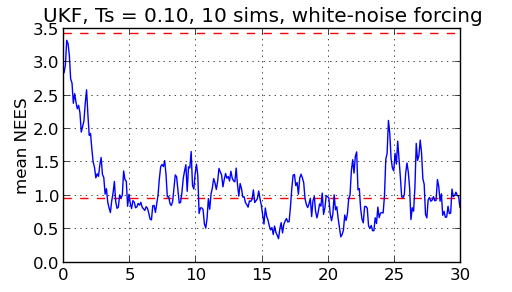
\includegraphics[width=0.49\textwidth]{../../challenge_problem/trials/nees_ukf_sims_01_medium}
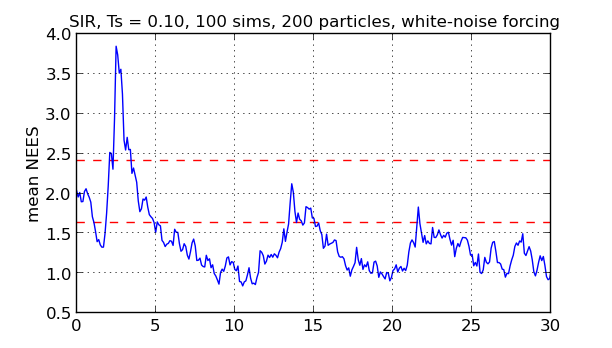
\includegraphics[width=0.49\textwidth]{../../challenge_problem/trials/nees_sir_200_sims_01_medium}
\caption{Mean NEES time histories for the pure white noise forcing cases.}
\label{fig:nees_01_medium}
\end{figure}

\begin{figure}[p!]
\centering
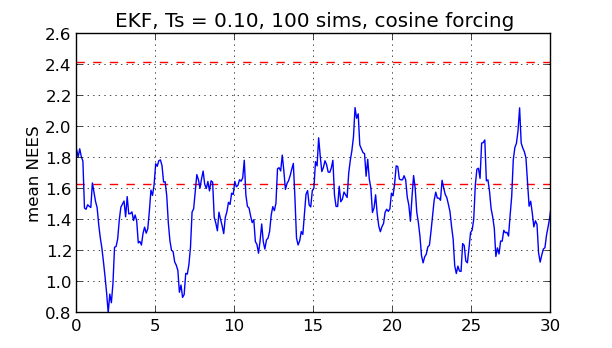
\includegraphics[width=0.49\textwidth]{../../challenge_problem/trials/nees_ekf_sims_10_medium}
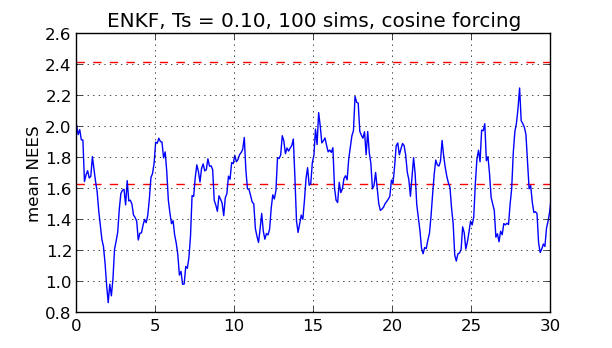
\includegraphics[width=0.49\textwidth]{../../challenge_problem/trials/nees_enkf_sims_10_medium}
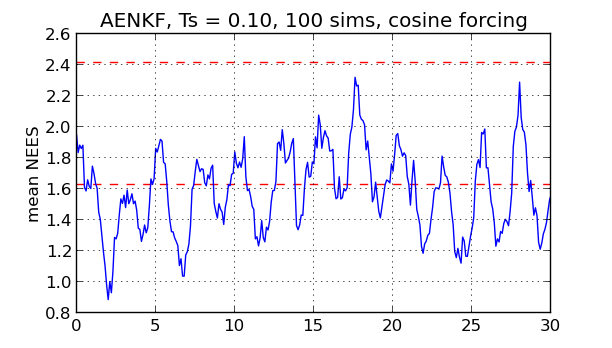
\includegraphics[width=0.49\textwidth]{../../challenge_problem/trials/nees_aenkf_sims_10_medium}
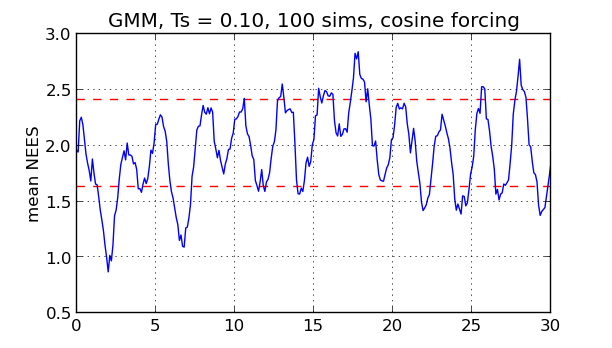
\includegraphics[width=0.49\textwidth]{../../challenge_problem/trials/nees_gmm_sims_10_medium}
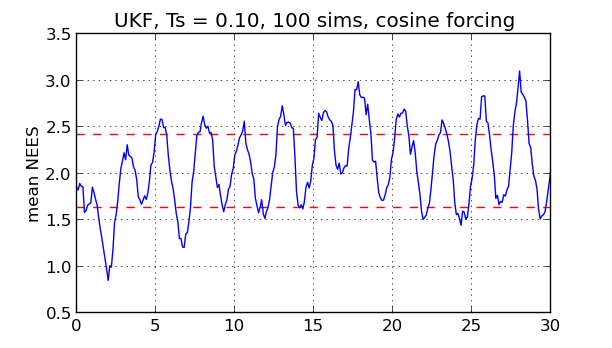
\includegraphics[width=0.49\textwidth]{../../challenge_problem/trials/nees_ukf_sims_10_medium}
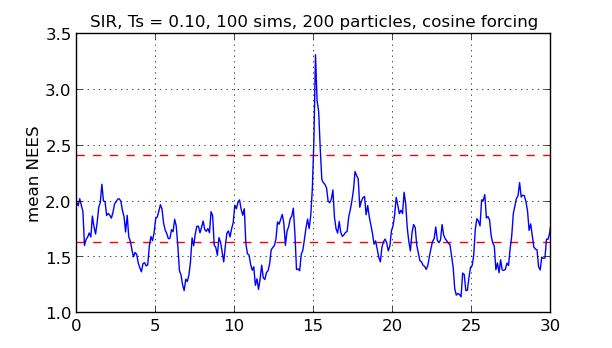
\includegraphics[width=0.49\textwidth]{../../challenge_problem/trials/nees_sir_200_sims_10_medium}
\caption{Mean NEES time histories for the pure cosine forcing cases.}
\label{fig:nees_10_medium}
\end{figure}

\begin{figure}[p!]
\centering
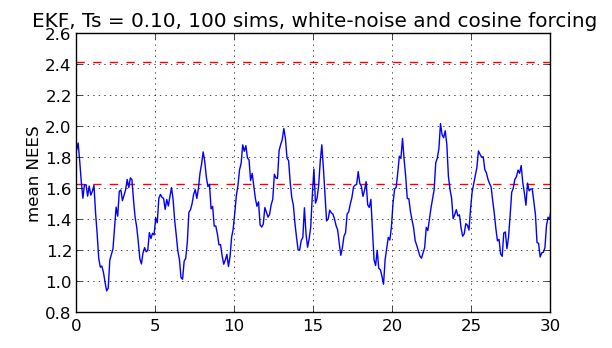
\includegraphics[width=0.49\textwidth]{../../challenge_problem/trials/nees_ekf_sims_11_medium}
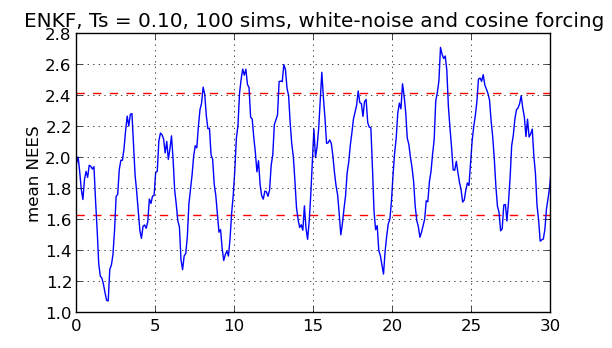
\includegraphics[width=0.49\textwidth]{../../challenge_problem/trials/nees_enkf_sims_11_medium}
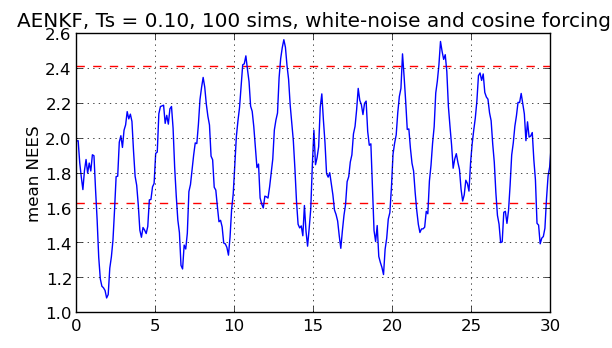
\includegraphics[width=0.49\textwidth]{../../challenge_problem/trials/nees_aenkf_sims_11_medium}
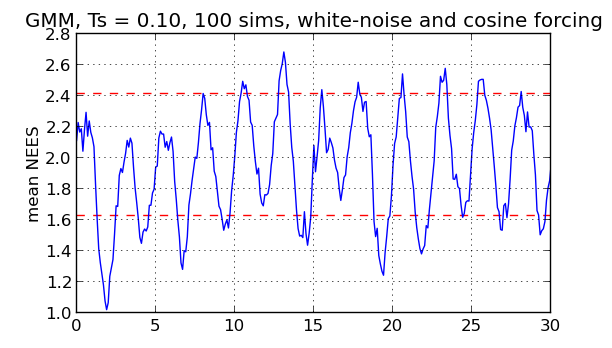
\includegraphics[width=0.49\textwidth]{../../challenge_problem/trials/nees_gmm_sims_11_medium}
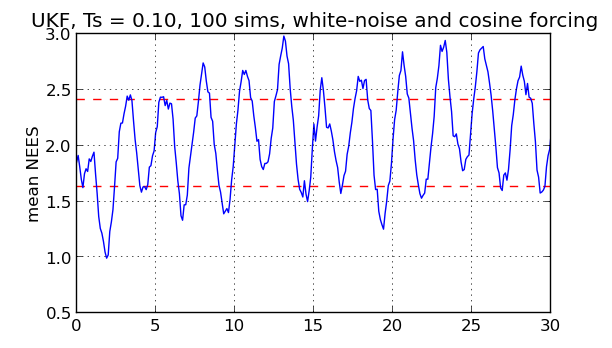
\includegraphics[width=0.49\textwidth]{../../challenge_problem/trials/nees_ukf_sims_11_medium}
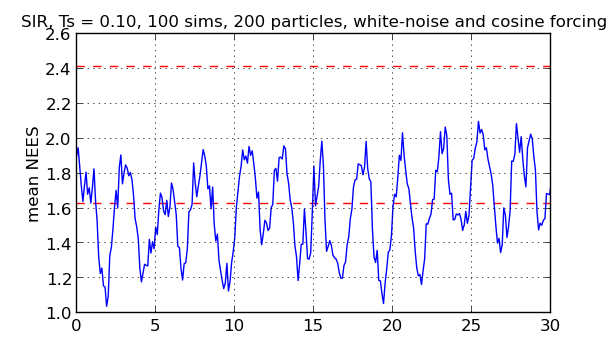
\includegraphics[width=0.49\textwidth]{../../challenge_problem/trials/nees_sir_200_sims_11_medium}
\caption{Mean NEES time histories for the pure cosine forcing cases.}
\label{fig:nees_11_medium}
\end{figure}

\subsubsection{Slow sample rate}

With the sample period of $T_s = 1.0$ seconds, the filters begin to experience the effects of bifurcation and large covariance growth during the propagation step; however, the non-ambiguous measurements enable the filters to remain stable, and any bimodal effects are largely manageable. 

For the case of purely Gaussian forcing, best performance in terms of MSE is obtained with the SIR, followed by the ENKF, EKF, GMM, and UKF.  In terms of consistency, all the filters are quite conservative, with the GMM having probably the most consistency performance. This reflects the effect of the long propagation time and underlying system bimodality on these unimodal filters. Of note, the lowest MSE seems to correlate with the greatest degree of conservatism in the results.

For the case of pure cosine forcing, lowest MSE is found with the ENFK, followed by the EKF, GMM, UKF, then SIR. The ENKF is extremely conservative again; the EKF, UKF, and GMM also have notable conservative and optimistic fractions. As in the medium sample rate, the SIR has higher MSE but apparently better consistency compared to the other filters.

For the case of mixed Gaussian and cosine forcing, lowest MSE is achieved with the ENKF, followed by the EKF, GMM, SIR, and UKF. Of these, the EKF and GMM are most conservative. The ENKF is the most optimistic, despite its relatively low errors. As might be expected from previous trials, the EKF tends to be conservative, the UKF switches between conservative and optimistic, and the SIR has good consistency.

%************************************************
% Performance table at Ts =  1.000000 with namebit 1
\begin{table}[h!]
\centering
\begin{tabular}{|c|c|c|c|c|}
\hline
Filter & $\mathrm{MSE}_1$ & $\mathrm{MSE}_2$ & Conservative fraction & Optimistic fraction \\
\hline
EKF &   0.6558 &   0.9599 &   0.3548 &  0.03226 \\
\hline
ENKF &   0.6215 &    0.822 &   0.4516 &        0 \\
\hline
AENKF &   0.6724 &    1.223 &   0.3636 &   0.1818 \\
\hline
GMM &   0.6822 &    1.042 &   0.1935 &  0.09677 \\
\hline
UKF &   0.7445 &    1.094 &   0.3871 &  0.06452 \\
\hline
SIR &   0.6023 &   0.7245 &   0.4516 &        0 \\
\hline
\end{tabular}
\caption{Performance metrics comparison of all filters with $T_s$ = 1.00 sec and Gaussian forcing term}
\label{table:compare_case_1_sample_2}
\end{table}


%************************************************
% Performance table at Ts =  1.000000 with namebit 2
\begin{table}[h!]
\centering
\begin{tabular}{|c|c|c|c|c|}
\hline
Filter & $\mathrm{MSE}_1$ & $\mathrm{MSE}_2$ & Conservative fraction & Optimistic fraction \\
\hline
EKF &   0.5854 &    1.104 &   0.2903 &  0.03226 \\
\hline
ENKF &   0.5671 &   0.9629 &   0.7419 &        0 \\
\hline
AENKF &   0.7642 &     2.19 &        0 &   0.5455 \\
\hline
GMM &   0.6128 &    1.219 &   0.2258 &        0 \\
\hline
UKF &   0.6316 &    1.128 &   0.2903 &   0.1613 \\
\hline
SIR &   0.7376 &    2.383 &        0 &  0.09091 \\
\hline
\end{tabular}
\caption{Performance metrics comparison of all filters with $T_s$ = 1.00 sec and cosine forcing term}
\label{table:compare_case_2_sample_2}
\end{table}


%************************************************
% Performance table at Ts =  1.000000 with namebit 3
\begin{table}[h!]
\centering
\begin{tabular}{|c|c|c|c|c|}
\hline
Filter & $\mathrm{MSE}_1$ & $\mathrm{MSE}_2$ & Conservative fraction & Optimistic fraction \\
\hline
EKF &   0.6076 &    1.077 &   0.2258 &  0.06452 \\
\hline
ENKF &   0.5749 &   0.9027 &   0.7419 &        0 \\
\hline
AENKF &   0.6698 &    1.321 &   0.1613 &        0 \\
\hline
GMM &   0.6394 &    1.195 &   0.5484 &        0 \\
\hline
UKF &    0.661 &    1.116 &   0.1613 &   0.2258 \\
\hline
SIR &   0.6756 &    1.035 &   0.1613 &  0.03226 \\
\hline
\end{tabular}
\caption{Performance metrics comparison of all filters with $T_s$ = 1.00 sec and Gaussian and cosine forcing terms}
\label{table:compare_case_3_sample_2}
\end{table}

\bibliographystyle{plain}
\bibliography{ref}

\end{document}
